% !TEX TS-program = xelatex
% !TEX encoding = UTF-8 Unicode

\documentclass{beamer}
\usepackage[fleqn]{amsmath}
%\usepackage{xfrac}%amsmath用来支持AMS-LaTex的数学功能 

\usepackage{ifxetex}

\usepackage[space]{ctex}

\ifxetex
	\usepackage{fontspec} % Font selection for XeLaTeX; see fontspec.pdf for documentation
	\defaultfontfeatures{Mapping=tex-text} % to support TeX conventions like ``---''
	\usepackage{xunicode} % Unicode support for LaTeX character names (accents, European chars, etc)
	\usepackage{xltxtra} % Extra customizations for XeLaTeX
\else
	\usepackage[T1]{fontenc}
   \usepackage[utf8]{inputenc}
\fi

\usepackage{relsize,fancyvrb}

\usepackage{tikz}
	\usetikzlibrary{arrows,shapes,shadows,mindmap}
\usepackage{graphicx}	%grapgics
\usepackage{multicol}
%\hypersetup{colorlinks=false} %不使用beamer默认的颜色(红色)
\mode<presentation>
{
  %\usetheme{Manhattan}
  \usetheme{Miun}
  % or ...
  \setbeamercovered{transparent}
  % or whatever (possibly just delete it)
}

\usepackage[english]{babel}
\usepackage{hyperref}
\usepackage{cite}
% or whatever

\ifxetex
	\setmainfont{Palatino Linotype} % set the main body font (\textrm), 
	\setsansfont{Gill Sans MT}
\else
% use default beamer font
\fi


\title%[Short Paper Title] % (optional, use only with long paper titles)
{Discussion About \\ D.A. \&  M.L.}

%\subtitle{Subtitle} % (optional)

\author%[] (optional, use only with lots of authors)
{Miao Feng}

\date% (optional)
{\today}

\subject{Talks}
% This is only inserted into the PDF information catalog. Can be left
% out. 

% Delete this, if you do not want the table of contents to pop up at
% the beginning of each subsection:
%\AtBeginSubsection[]
%{
%  \begin{frame}<beamer>{Outline}
%    \tableofcontents[currentsection,currentsubsection]
%  \end{frame}
%}

\AtBeginSection[]
{
    \begin{frame}<beamer>{Outline}
        \tableofcontents[currentsection,hideallsubsections]
    \end{frame}
}
\AtBeginSubsection[]
{
    \begin{frame}<beamer>{Outline}%[shrink]
        \tableofcontents[sectionstyle=show/shaded,subsectionstyle=show/shaded]
    \end{frame}
}

% If you wish to uncover everything in a step-wise fashion, uncomment
% the following command: 

%\beamerdefaultoverlayspecification{<+->}

\begin{document}

%====================================================================%
%====================================================================%

\begin{frame}
  \titlepage
\end{frame}

%====================================================================%
\section*{Before}
%====================================================================%
% ----------------slide的结构开始---------------- %
\begin{frame}{Before I start}

  Theme:\textbf{机器学习与资料同化的关系}\\
  P.S.:根据个人理解、在哈工大的学习整理所得。\\
  Inferences: \\
\footnotesize{
\begin{itemize}
  \item
	\begin{thebibliography}{99}
	\bibitem[周志华, 2016]{p1} 周志华 (2016), \textbf{机器学习}
	\end{thebibliography}
  \item
	\begin{thebibliography}{99} 
	\bibitem[李航,2012]{p1} 李航(2012),\textbf{统计学习方法}
%\newblock Title of the publication. \emph{Journal Name} 12(3), 45 -- 678.
	\end{thebibliography}
  \item
	\begin{thebibliography}{99} 
	\bibitem[邹晓蕾, 2009]{p1} 邹晓蕾(2009), \textbf{资料同化理论与应用}
	\end{thebibliography}
\end{itemize}
}
B.T.W.:You may find many errors in this report,please help me correct it.
\end{frame}
% ----------------slide的结构结束---------------- %
%====================================================================%

\section{Basics of M.L. }
%====================================================================%
\subsection{What\rq{}s M.L.}
% ----------------slide的结构开始---------------- %
\begin{frame}{What\rq{}s M.L.}{\quad\quad\quad M.L.,D.L.,S.L.}
%====================================================================%

% ----------------分栏的结构开始---------------- %

\begin{columns}

\column{.7\textwidth}

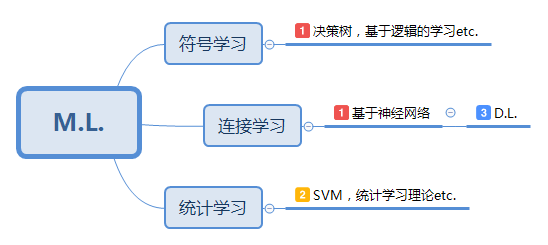
\includegraphics[scale=0.4]{fig/ML.png}

\column{.3\textwidth}


  \begin{enumerate}
  \item 1980s\textasciitilde 1990s 中期 
  \item 1990s中期\textasciitilde
  \item 2000s\textasciitilde
  \end{enumerate}
\end{columns}
% ----------------分栏的结构结束---------------- %
\end{frame}
% ----------------slide的结构结束---------------- %
%====================================================================%

% ----------------slide的结构开始---------------- %
\begin{frame}{What\rq{}s M.L.}{\quad\quad\quad M.L.,D.L.,S.L.}
%====================================================================%
  \begin{block}{Definition}
   \begin{itemize}
  \item M.L.
	\begin{enumerate}
	\item Mitchell:对于某类任务T和性能度量P,如果一个计算机程序在T上以P衡量的性能随着经验E而自我完善,那么我们称这个计算机程序在从经验E学习。
	\item Samuel:在不直接针对问题进行编程的情况下,赋予计算机学习能力的一个研究领域。
	\end{enumerate}
  \item D.L.\\狭义:多层神经网络
  \end{itemize}
  \end{block}
\end{frame}
% ----------------slide的结构结束---------------- %

% ----------------slide的结构开始---------------- %
\begin{frame}{What\rq{}s M.L.}{\quad\quad\quad S.L.,D.M.}
%====================================================================%

  \begin{block}{Definition}
   \begin{itemize}
  \item S.L.\\统计学习,基于数据构建概率统计模型并运用模型对数据进行预测与分析
  \item D.M.\\数据挖掘,指从大量的数据中通过算法搜索隐藏于其中信息的过程。算法主要使用M.L.的,但是重在数据中隐含的信息
  \end{itemize}
  \end{block}
\end{frame}
% ----------------slide的结构结束---------------- %


% ----------------slide的结构开始---------------- %
\begin{frame}{What\rq{}s M.L.}{\quad\quad\quad Forget things before}
%====================================================================%

  \begin{block}{Be simple}
   \begin{itemize}
  \item M.L.基于数据进行模型训练,最终归纳出一个面向一种性能度量的决策。
  \item M.L.现在的主流算法是基于连接主义的D.L.和基于统计学习的SVM、KNN、logistics回归、EM、AdaBoost等
  \end{itemize}
  \end{block}
\end{frame}
% ----------------slide的结构结束---------------- %


% ----------------slide的结构开始---------------- %
\begin{frame}{What\rq{}s M.L.}{\quad\quad\quad Classifications}
%====================================================================%
% ----------------分栏的结构开始---------------- %

\begin{columns}

\column{.6\textwidth}

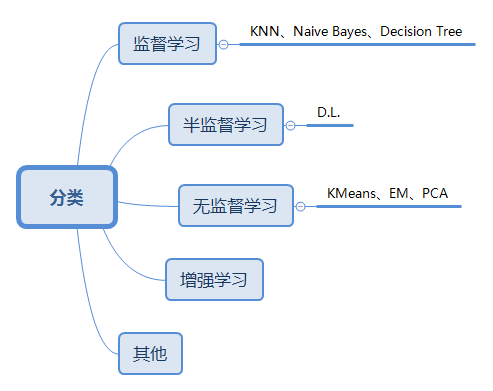
\includegraphics[scale=0.45]{fig/Class.png}

\column{.4\textwidth}

   \begin{itemize}
  \item 监督学习\\测试集带label。
  \item 半监督学习\\测试集部分带label。
  \item 无监督学习\\测试集不带label。
  \item 增强学习\\没有规则化的数据集,多用于A.I.中机器人控制
  \end{itemize}

\end{columns}
% ----------------分栏的结构结束---------------- %
\end{frame}
% ----------------slide的结构结束---------------- %


%====================================================================%
\subsection{M.L. Theory}

%====================================================================%

% ----------------slide的结构开始---------------- %
\begin{frame}{M.L. Theory}{\quad \quad\quad Problem Definition}
%====================================================================%
 \begin{block}{Definition}
   \begin{itemize}
  \item 样本点(数据集)\\输入数据与输出数据组成的样本对。数据集分为\textbf {训练集}与\textbf{测试集}。输出数据又被称为\textbf {label}。训练集用于训练模型,测试集用于测试训练得到的模型的性能。
  \item 模型\\输入空间到输出空间的一个映射
  \end{itemize}
  \end{block}
  \end{frame}

%====================================================================%
% ----------------slide的结构开始---------------- %
\begin{frame}[fragile]{M.L. Theory}{\quad \quad\quad Still boring,try something practical}
%====================================================================%
\begin{block}{}
已知辐射值$R=( r_1,r_2,r_3,\ldots , r_n )^T$,对应温度为\\
$T=(t_1,t_2,t_3,\ldots , t_n )^T$,欲知$R\rq{}=( r_{n+1},r_{n+2},r_{n+3},\ldots , r_N )^T$时对应的温度\\
\end{block}
以辐射值为输入数据,温度为输出数据,则\\样本对:$Y=\{[R \quad R\rq{}],T\}$ \\ 训练集:$Y_1=\{R,T\}$ \\ 测试集:$Y_2=\{R\rq{},[ \quad ]\}$\\label:$T=(t_1,t_2,t_3,\ldots , t_n )^T$\\
得到的模型等价于GMF

\end{frame}
% ----------------slide的结构结束---------------- %
%====================================================================%

% ----------------slide的结构开始---------------- %
\begin{frame}{M.L. Theory}{\quad \quad\quad Methods}
%====================================================================%

\includegraphics[scale=.45]{fig/charcter.png}

\end{frame}
% ----------------slide的结构结束---------------- %

%====================================================================%

% ----------------slide的结构开始---------------- %
\begin{frame}{M.L. Theory}{\quad \quad\quad ERM,SRM,Goal}
%====================================================================%
\begin{enumerate}
  \item ERM,说明与训练集的数据拟合的很好
  \item SRM,说明对测试集的预测效果很好,比如对已知的辐射值推测温度
  \item 目标:最小化结构风险的同时保证经验风险最小,即确保模型的泛化能力,在符合策略条件的众多模型中挑选最普适的模型
  \end{enumerate}  
  \quad \quad Therefore,we\rq{}d like to keep an eye on the \textbf{regularization}


\end{frame}
%====================================================================%
% ----------------slide的结构开始---------------- %
\begin{frame}[t]{M.L. Theory}{\quad \quad\quad Rules of choosing model}
%====================================================================%
\textbf{Priciple}:奥斯卡姆剃刀(Oscam's razor),所有符合条件的模型中,模型越简单,泛化性能越好\\
\textbf{Methods}:$
%\begin{equation*}
 \underbrace{\textbf{正则化}}_{\text{模型添加penalty}} +\quad  \underbrace{\textbf{交叉验证}}_{\text{数据集trick}}$
%\end{equation*}


\begin{block}{Regularization}
\begin{equation}
\min\limits_{f \in \mathcal{F}}\underbrace{\frac{1}{N}\sum_{i=1}^N L(y_i,f(x_i))}_{\text{经验风险(loss function) }}+ \underbrace{ \lambda R(f)}_{\text{penalty}}\quad \lambda \geq 0
\end{equation}

其中,$\lambda$调节经验风险与正则化项之间的关系\\
$R(f)$ \textbf{depends on your problems},常用的有$\ell_0,\ell_1,\ell_2,\ell_p,\ell_\infty $

\end{block}
\end{frame}
% ----------------slide的结构结束---------------- %
%====================================================================%
% ----------------slide的结构开始---------------- %
\begin{frame}{M.L. Theory}{\quad \quad\quad Rules of choosing model}
%====================================================================%
\begin{block}{Cross Validation}
\begin{itemize}
\item 思想\\重复利用数据
\item 方法\\将给定数据切分组合为训练集与测试集,在此基础上反复训练、测试以及模型选择
\item 分类\\简单交叉验证、S折法、留一法
\end{itemize}
\end{block}
\end{frame}

%====================================================================%

%====================================================================%
\subsection{Some M.L.algorithms}
%====================================================================%

% ----------------slide的结构开始---------------- %
\begin{frame}{Some M.L. algorithms}{\quad \quad \quad Bayesian Framework}
%====================================================================%
%====================================================================%
% ----------------分栏的结构开始---------------- %

\includegraphics[scale=.45]{fig/Bayes.png}


   \begin{itemize}
  \item 近似推断:避免精确推断的高计算需求
  \end{itemize}

\end{frame}
% ----------------slide的结构结束---------------- %
%====================================================================%

% ----------------slide的结构开始---------------- %
\begin{frame}{Some M.L. algorithms}{\quad \quad \quad Bayesian Framework}
%====================================================================%

   \begin{itemize}
  \item 采样法\\多采用马尔科夫链蒙特卡洛采样。当采样足够多时,认为可以近似表达分布,目标是直接通过采样计算期望
  \item 变分推断\\使用已知简单分布逼近需推断的复杂分布,并通过限制近似分布的类型,得到一局部最优但有确定解的近似后验分布。e.g. 高斯分布
  \item EM算法\\期望最大化算法。原理为MAP(最大化后验概率)。分E步和M步,E步求似然期望,M步寻找能使E步产生的似然期望最大化的参数值。即,最大似然(ML)
  \end{itemize}
\end{frame}
% ----------------slide的结构结束---------------- %
%====================================================================%

% ----------------slide的结构开始---------------- %
\begin{frame}{Some M.L.algorithms}{\quad \quad \quad Linearity Regression}
%====================================================================%

\begin{block}{}
已知输入数据$X$,输出数据$Y$,求解$\theta$
\begin{equation}
f_{\theta}(X)={\theta}^TX
\end{equation}
%方法:
\begin{equation}
\arg\min\limits_{\theta} J_{\theta}(X)+\lambda R(\theta) 
\end{equation}
\begin{equation}
J_\theta(X)=\sum_{i=1}^N (f_{\theta}(x^{(i)})-y^{(i)})^2
\end{equation}

\begin{equation*}
(4) +
\begin{cases} 
0,  & \mbox{if }\lambda \mbox{ = 0}\Rightarrow OLS \\
\lambda \left \| \theta \right \|_1, & \mbox{if } \lambda \mbox{ >0}\Rightarrow LASSO \\
\lambda \left \| \theta \right \|_2^2, & \mbox{if } \lambda \mbox{ >0} \Rightarrow Ridge
\end{cases}
\end{equation*}

\end{block}

\end{frame}
% ----------------slide的结构结束---------------- %
%====================================================================%

% ----------------slide的结构开始---------------- %
\begin{frame}{Some M.L.algorithms}{\quad \quad \quad Linear Regression}
%====================================================================%

 (4)根据loss function定,平方loss+问题overdetermined $\Rightarrow$ 最小二乘\\
  通常,$\ell_0,\ell_1$比$\ell_2$稀疏性好,所得模型泛化能力更强,但是$\ell_0,\ell_1$优化求解不如$\ell_2$简单

\end{frame}
% ----------------slide的结构结束---------------- %
%====================================================================%

% ----------------slide的结构开始---------------- %
\begin{frame}{Some M.L.algorithms}{\quad \quad \quad Others:Many!!}
%====================================================================%
%\begin{block}{}
\begin{itemize}
\item 核技巧(kernel tricks)以及相关的支持向量机(SVM)、高斯过程回归(GPR)等算法
\item 神经网络(ANN)和D.L.. e.g.: CNN、RNN
\item 降维算法,e.g. 主成分分析(PCA)
\item and so on and so forth
\end{itemize}
%\end{block}

\end{frame}
% ----------------slide的结构结束---------------- %

%====================================================================%

\section{The relationship of M.L.\& D.A.}
%====================================================================%
\subsection {Why talking about this?}
%====================================================================%
% ----------------slide的结构开始---------------- %
%====================================================================%
\begin{frame}{Why talking about this?}{\quad \quad \quad It\rq{}s not nonsense}
May I could say the Theory of D.A. comes from \textbf{control theory},using \textbf{PDE,ODE} to make a perfect description of the natural phenomena,although it\rq{}s \textbf{impossible}.\\The natural phenomena is too complicated to describe , we need to \textbf{simplify} it again and again.Afterwards,we get our model, within plenty of \textbf{biases,errors}.\\
M.L. focuses on the \textbf{general model}.You just need to spend more time on the \textbf{mapping} between the input data and output data, without much consideration about the physics,biology etc.And it did works. 
\end{frame}

% ----------------slide的结构结束---------------- %
%====================================================================%
% ----------------slide的结构开始---------------- %
%====================================================================%
\begin{frame}{Why talking about this?}{\quad \quad \quad It\rq{}s not nonsense}

Then why didn\rq{}t us try to keep an eye on the more general model without considering many physics process? \\
In fact, we are doing it. The \textbf{statistics} in D.A. supports me. If you look at Particle Filter,Hierarchical Bayesian network, you will find more.

We are \textbf{combining D.A.and M.L.}.\\
But we need to be better.
\end{frame}

% ----------------slide的结构结束---------------- %
%====================================================================%

\subsection{Mathematical Basis}
%====================================================================%
% ----------------slide的结构开始---------------- %
%====================================================================%

\begin{frame}{Mathematical Basis}{\quad \quad \quad you may need to learn}
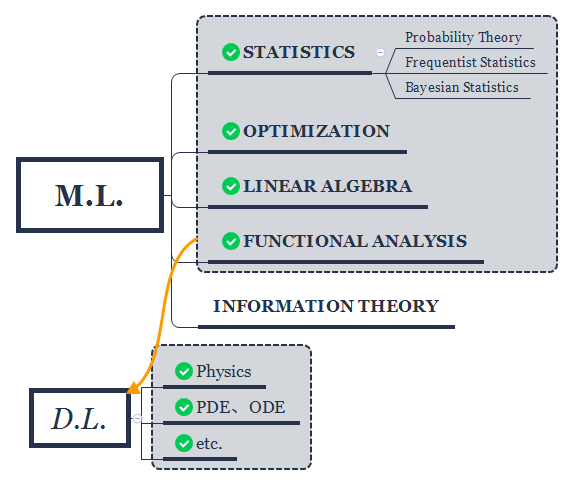
\includegraphics[scale=.42]{fig/math.png}
\end{frame}

% ----------------slide的结构结束---------------- %

%====================================================================%
\subsection{Methods}
%====================================================================%
% ----------------slide的结构开始---------------- %
\begin{frame}{Methods}{\quad \quad \quad Let\rq{}s go back firstly}
%====================================================================%

\includegraphics[scale=.45]{fig/Bayes.png}

According to the figure above, I\rq{}d like to make some extensions.

\end{frame}
% ----------------slide的结构结束---------------- %

%====================================================================%
% ----------------slide的结构开始---------------- %
\begin{frame}{Methods}{\quad \quad \quad D.A. Framework,from the perspective of M.L.}
% ----------------分栏的结构开始---------------- %
\begin{columns}

\column{.8\textwidth}

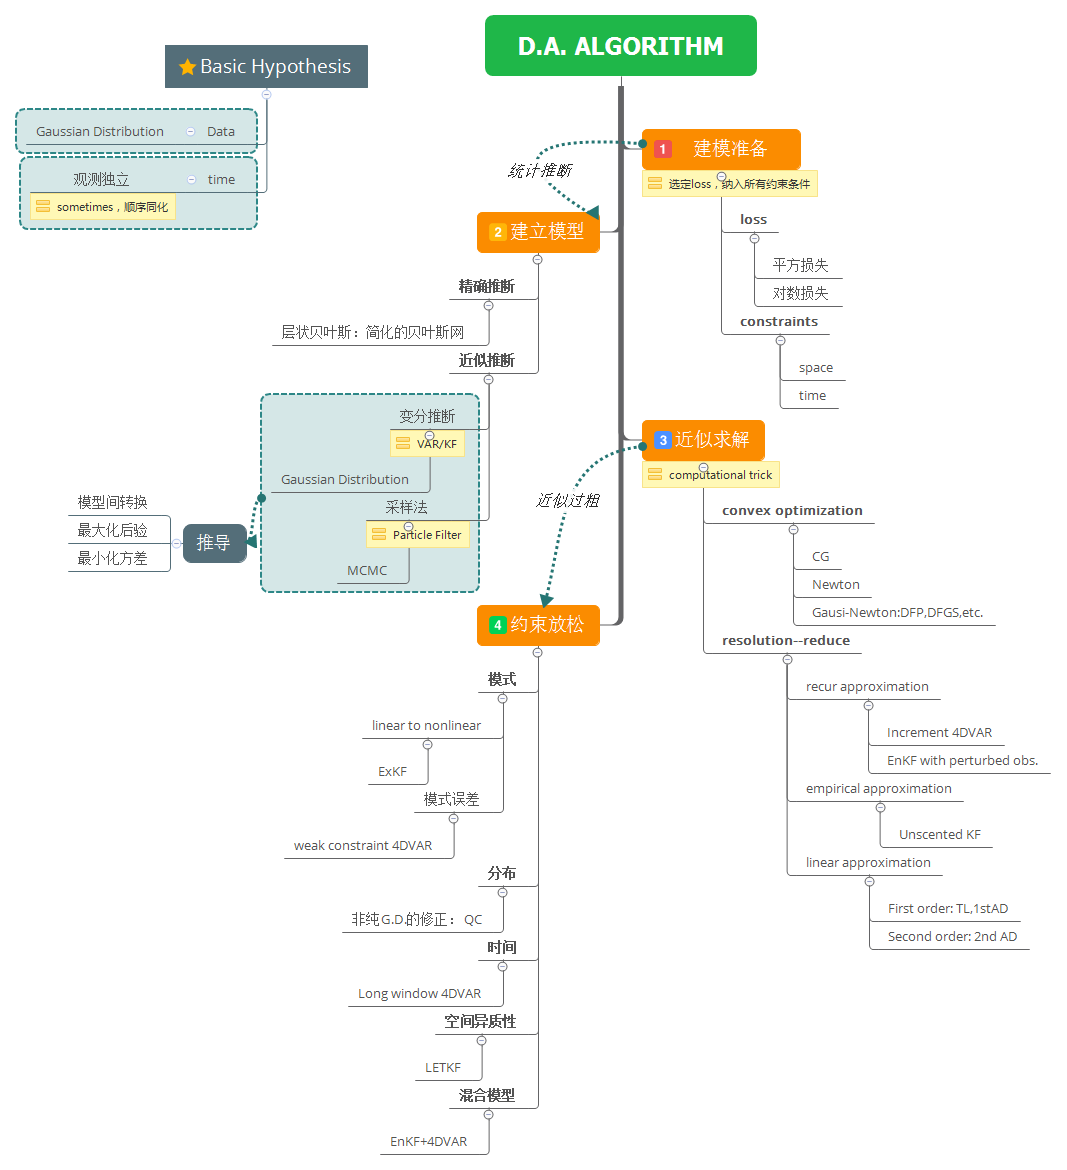
\includegraphics[scale=.18]{fig/daalg.png}

\column{.2\textwidth}

Just for an instance, as for I\rq{}m a green hand in D.A.\& M.L., you may find many errors in it

\end{columns}

% ----------------分栏的结构结束---------------- %

\end{frame}

% ----------------slide的结构结束---------------- %

%====================================================================%

%====================================================================%
% ----------------slide的结构开始---------------- %
\begin{frame}{Methods}{\quad \quad \quad change the perspective}

\begin{block}{from 邹晓蕾,\emph{资料同化与应用}page43}
3DVAR、4DVAR、EnKF,分析增量均为观测增量的加权平均。不同的D.A.方法只是获得的后验权重$(W)$估计不同,所有的推导都是下式的直接或间接的表达
\begin{equation}
x^{a}=x^b+W(y^o-y)
\end{equation}
\end{block}
参考线性回归,to be \textbf{more general},可以增加\textbf{正则项}
%\begin{block}{from John M. Lewis \emph{Dynamic D.A.} page 115}--Tikhonov regularization
%an unified model solve both the under-determined and over-determined problems
%\begin{equation}
%f(x)=\frac{\alpha}{2}x^Tx+\frac{1}{2}\left \| (z-Hx) \right \|^2
%\end{equation}
%
%\end{block}

\end{frame}

% ----------------slide的结构结束---------------- %
%====================================================================%
% ----------------slide的结构开始---------------- %
\begin{frame}{Methods}{\quad \quad \quad Tikhonov regularization}

\begin{block}{from John M. Lewis \emph{Dynamic D.A.} page 115}
an unified model which solve both the under-determined and over-determined problems
\begin{equation}
f(x)=\frac{1}{2}\left \| (z-Hx) \right \|^2+\frac{\alpha}{2}x^Tx
\end{equation}

\end{block}
What if changing the norm to $\ell_0,\ell_1$ norm, will it make sense?

A.K.A. \emph{Will the $\ell_0,\ell_1$ norm,which is popularly used in M.L.,help us get a more general model in D.A. ?? }
\end{frame}

% ----------------slide的结构结束---------------- %


%%====================================================================%
%\section{An experience:failed}
%
%%====================================================================%
%
%\begin{frame}{An experience:failed}{\quad \quad \quad Just show the importance of D.A. and Physics}
%
%\begin{block}{}
%
%Task:雷达数据预测未来降水\\
%讲一下自己做的和人家实验的对比\\说明:1.单纯算法不够。。2. 深度学习的结合训练效果
%
%\end{block}
%
%
%\end{frame}
%
%% ----------------slide的结构结束---------------- %


%====================================================================%
\section{Some issues}

%====================================================================%

\begin{frame}{Some issues}{\quad \quad \quad Some problems in D.A. }


Problems in D.A.
\begin{itemize}
\item 计算需求
\item 模式误差
\item 观测误差(数据集)
\item 观测独立假设(实际不全为真)
\item 预报性
\end{itemize}

\end{frame}

% ----------------slide的结构结束---------------- %
%====================================================================%
% ----------------slide的结构开始---------------- %
\begin{frame}{Some issues}{\quad \quad \quad Just for an example}
You may get some inspirations from M.L.

\begin{itemize}
\item 计算需求$\Leftarrow$ 降维:kernel trick,sparse matrix reconstruction
\item 模式误差$\Leftarrow$ D.L.是否可以与模式结合??LSTM擅长分析时间序列
\item 观测误差(数据集)$\Leftarrow$ D.M.中的分箱、回归、离群点检测etc.
\item 观测独立假设(实际不全为真)$\Leftarrow$ 随机过程取代随机变量:GPR?LSTM?
\item 预报性(a.k.a.泛化性能) $\Leftarrow$ 正则化:norm selection
\end{itemize}

\end{frame}

% ----------------slide的结构结束---------------- %
%====================================================================%

% ----------------slide的结构开始---------------- %
\begin{frame}{Some issues}{\quad \quad \quad You may be interested in }

Data need huge storage space.\\
\textbf{Hadoop and Spark} works well in the D.M. of big data

\begin{block}{}
\begin{enumerate}
\item Hadoop:Apache的项目,分布式系统架构,开源。下设HDFS、HBase、map/reduce等子项目。
\begin{itemize}
 \item HDFS实现对于大数据的分布式文件存储。
 \item HBase不同于Mysql、SQLSERVER、Oracle等关系型数据库,是No-sql数据库。擅长文件数据存储检索。常用的no-sql数据库还有mongoDB。
 \item map/reduce为数据并行计算框架,用于作业调度。map步将大作业分散为小作业,reduce步将小作业的输出结果组织为最终结果。
\end{itemize}
\end{enumerate}
\end{block}
\end{frame}
% ----------------slide的结构结束---------------- %
%====================================================================%

%% ----------------slide的结构开始---------------- %
\begin{frame}{Some issues}{\quad \quad \quad You may be interested in }

\begin{block}{}	%注意,这里的{}不可少。。不然编译会报错
\begin{enumerate}
\item Spark:Apache项目,由UC Berkeley AMP lab开发的类map/reduce的通用并行框架,开源。\\M.L.的可行框架之一,计算速率优于map/reduce。\\可以在HDFS中并行运行,且提供M.L.的API。也可单独运行。

\item Ray:由UC Berkeley RISE Lab开发,尚在开发中。旨在让基于Python的M.L.和D.L.工作负载能够实时执行,并具有类似消息传递接口(MPI)的性能和细粒度。据Michael I.Jordan说,Ray性能优于Spark,将取代Spark。
\end{enumerate}
\end{block}
B.T.W.\quad Michael I.Jordan曾先后担任AMP、RISE的顾问,Spark和Ray都有做指导。研究方向为统计学习

\end{frame}
% ----------------slide的结构结束---------------- %
%====================================================================%



\section{Summary}
%====================================================================%


% ----------------slide的结构开始---------------- %

\begin{frame}{Summary}{Outline again}

\begin{block}{relationship}
Algorithm:\\
\begin{enumerate}
\item Bayesian network
\item linear regression
\end{enumerate}

May be useful:\\
\begin{enumerate}
\item dimension reduce and sparse matrix reconstruction: kernel tricks,PCA
\item computation efficiency: D.L.,Ray
\item storage space: HDFS
\end{enumerate}

\end{block}

\end{frame}
% ----------------slide的结构结束---------------- %
%====================================================================%


\begin{frame}{Summary}{}
 The combination of D.A.\& M.L. is \huge{ \textbf{unavoidable}}

\end{frame}

\end{document}
 